\chapter{Mögliche Anwendungen von Strukturbatterien im Leichtbau}

Strukturbatterien könnten Anwednungen in zahlreichen Bereichen auf vielseitige Art und Weise eingesetzt werden. 

\begin{table}[ht]
    \centering
    \caption{\label{tab:pot_anwendungen}Potentielle Anwendungen von Strukturbatterien für verschiedene Einsatzbereiche.}
    \begin{tabular}{m{0.2\textwidth} m{0.2\textwidth}<{\centering} m{0.4\textwidth}<{\centering} m{0.2\textwidth}}
        \toprule
        Technologischer Einsatzbereich&Teilbereiche&Anwendungsbeispiele&Quelle\\
        \midrule
        \multirow{3}*{Luftfahrt}   &Tertiärestrukturen&Entertainmentsystem und Innenverkleidungen& \\
                    &Sekundärstruktur&Trennwände und Gepäckfächer; Fahrwerkstüren; Rahmenstrukturen und Stellklappem& \\
                    &Primärstrukturen&Flugzeugrumpf und Flügelstrukturen& \\
                    %\hspace{1em}
                    \hline
        \multirow{3}*{Automobil}   &Karosserieteile&Türverkelidungen, Innenraumelemente und Sitzstrukturen&\\
                    &Sekundäre Fahrzeugstrukturen&Armaturenebrett; Dachhimmel; Trennwände&\\
                    &Tragende Strukturen&Fahrgestell oder Karosserie&\\
                    \hline
        Innenraumelemente und Sitzstrukturen&\\
                    &Sekundäre Fahrzeugstrukturen&Armaturenebrett; Dachhimmel; Trennwände&\\
                    &Tragende Strukturen&Fahrgestell oder Karosserie&\\
        \bottomrule
    \end{tabular}
\end{table}

\section{Roadmap}
Eine Abschätzung 


\section{Potenzial für den Flugzeugkabineninnenraum}

\begin{figure}[!h]
	%\raggedleft
		%\def\svgwidth{\columnwidth}
        \center
		\includegraphics[width=0.8\textwidth, angle=0]{Abbildungen/06_Leichtbau/cabine_usecase.pdf}
		\caption{\label{fig:cabin}Der Einsatz von Strukturbatterien kann in Flugzeugkabinen dazu eingesetz werden um eine kabelose Stromversorgung am Passagiersitz zu ermöglichen, was nicht nur Kabel einsparrt, sonder auch bei der Gewichtsverteilung hilft.}
\end{figure}

\section{Potenzial für die mobile Robotik}

\begin{figure}[!h]
	%\raggedleft
		%\def\svgwidth{\columnwidth}
        \center
		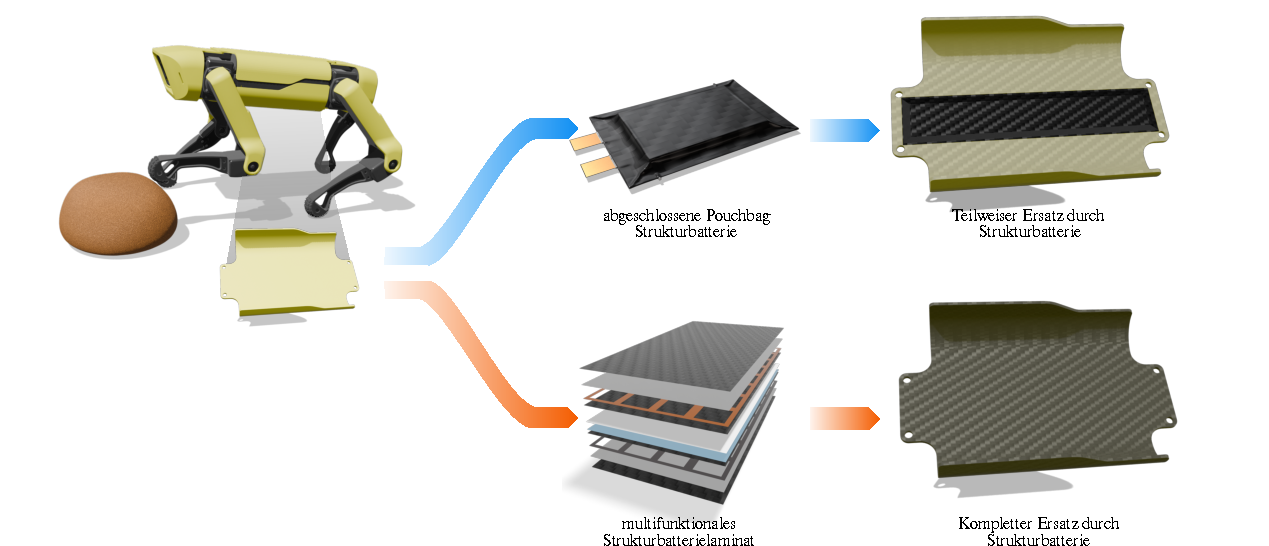
\includegraphics[width=0.99\textwidth, angle=0]{Abbildungen/06_Leichtbau/dog_robot_sb_study.pdf}
		\caption{\label{fig:robot_dog}In der mobilen Robotik können Strukturbatterien durch Integration bisher primaär Lastentragende Komponenten Integirert werden, um die Reichweite zu erhöhen.}
\end{figure}
